\documentclass[a4paper]{article}

\usepackage[swedish]{babel}
\usepackage[T1]{fontenc}
\usepackage[utf 8]{inputenc}
\usepackage{graphicx}

\begin{document}

\section*{Kvalitetsplan}

Kvalitén på produkten verifieras genom \textit{tester}.

Under projektets gång kommer det att utföras enhetstester för att testa de minsta delarna i systemet, funktionella tester på olika delar av systemet för att testa dess funktionalitet, prestandatester för att fastställa systemets prestanda och kapacitet, och slutligen användartester för att upptäcka förbättringar av systemet utifrån ett användarperspektiv.

Kvalitén på elektriska komponenter och övrig hårdvara kan verifieras genom tester med mätutrustning, medan en IDE (\textit{eng. Integrated Design Environment}) kan användas för att verifiera kvalitén på mjukvaran. Hur väl hård- och mjukvaran fungerar ihop verifieras genom funktionstester och användartester.

Utifrån de krav som specificeras i systembeskrivningen (se avsnitt nr) skrivs ett \textit{testfall} som testar om kravet är uppfyllt. Varje testfall består av följande data:

\begin{description}
  \item [ID] Ett unikt ID på formen TXnnnvm, där X är E, F, P eller A för enhetstest, funktionellt test, prestandatest respektive användartest, nnn är ett nummer mellan 0 och 999 tilldelat i den ordning testfallen skapats, och m är versionsnummret. Exempelvis är TF012v3 den tredje versionen av det tolfte funktionella testfallet.
  \item [Namn] Ett namn som tydligt beskriver vad testfallet ska testa.
  \item [Beskrivining] En beskrivning av testfallet. Beskrivningen ska beskriva syftet med testfallet, vilken komponent som testas, vilket eller vilka krav som testas samt eventuella tekniska förutsättningar för att genomföra testet.
  \item [Teststeg] De steg som måste utföras för att utföra testfallet.
  \item [Förväntat resultat] Beskrivning av det förväntade resultatet för testfallet.
\end{description}

Eftersom kvalitén på produkten verifieras genom tester är det viktigt att kvalitén på testfallen och utförandet av de är mycket hög. För att säkerställa att alla testfall som skrivs håller en hög kvalité ska skapandet och utförandet av testfallen ske enligt följande rutin.
I stunden ett testfall skapas tilldelas det automatiskt status \textit{Utkast}. Testfallet kan sedan skickas vidare till \textit{granskning}. Granskningen ska ske av åtminstone en (1) person och personen får inte ha varit inblandad i skrivandet av testfallet. Testfallet kan antingen bli \textit{godkänt} eller \textit{avfärdat}. Om testfallet blir godkänt ändras dess status till \textit{Klar för test} och det får köras. Ett föråldrat eller inaktuellt testfall kan skickas tillbaka till granskning. Om testfallet däremot blir avfärdat måste det revideras och sedan åter skickas till granskning. De två reglerna för att skapa och köra testfall är följande: (1) endast testfall med status Utkast får redigeras och (2) endast testfall som har blivit granskade och godkända får köras.

\begin{figure}[h]
  \centering
  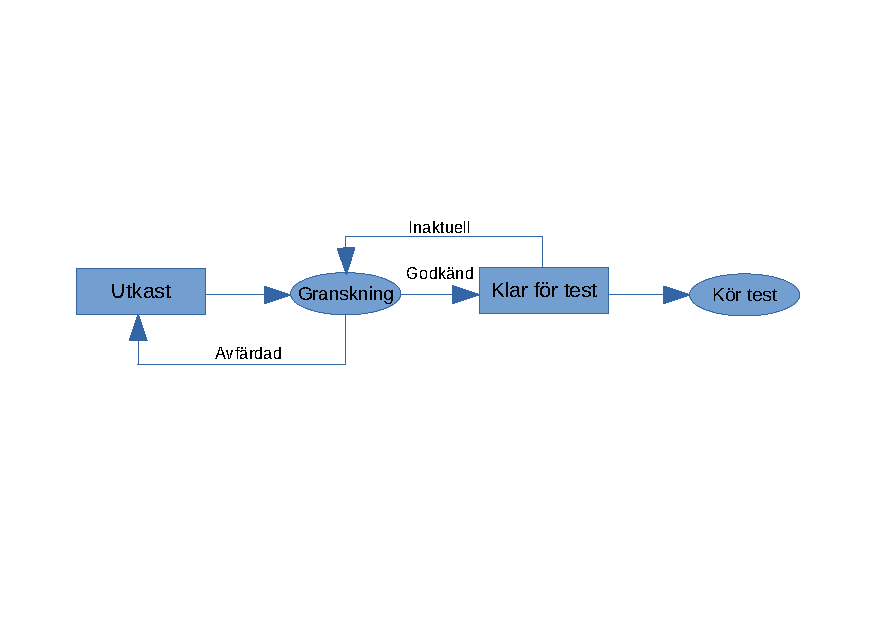
\includegraphics[trim={0 4cm 0 3cm}, clip, scale=0.8]{figurer/testrutin.pdf}
  \caption{Vår rutin kring att skriva och genomföra testfall.}
\end{figure}

Resultatet av samtliga körda tester ska sammanställas i en CSV-fil. I testresultatfilen ska följande fält, varav det sista är frivilligt, fyllas i:

\begin{description}
  \item [ID] Testfallets unika ID.
  \item [Namn] Testfallets namn.
  \item [Hårdvara] Hårdvara som använts vid utförandet av testet.
  \item [Mjukvara] Version på mjukvara som använts vid utförandet av testet.
  \item [Faktiskt resultat] Beskrivning av det faktiska resultatet om det skiljer sig mot det färväntade resultatet angivet i testfallet.
  \item [Status] Status på testet. \textit{G} ska anges om testet blev godkänt, det vill säga om det faktiska resultatet blev det samma som det förväntade resultatet, och \textit{M} om testet misslyckades.
  \item [Kommentar] Eventuella kommentarer, till exempel analys av testfallet. Detta fält är frivilligt.
\end{description}

Resultatet av samtliga körda tester ska analyseras och diskuteras åtminstone på det veckovisa gruppmötet. Då ska även bestämmas vilka tester som i första hand ska köras innan nästa möte.

\subsection*{Integrering av utveckling och testning}

Eftersom vår projektgrupp består av endast fem personer kan vi integrera testning med utveckling. Vi väljer att jobba efter en cirkulär modell där testningen blir en naturlig del av utvecklingsfasen, ty så snart en funktion utvecklats, testas den. På så sätt kan buggar hittas och lösas tidigt i utvecklingsfasen.

\begin{figure}[h]
  \centering
  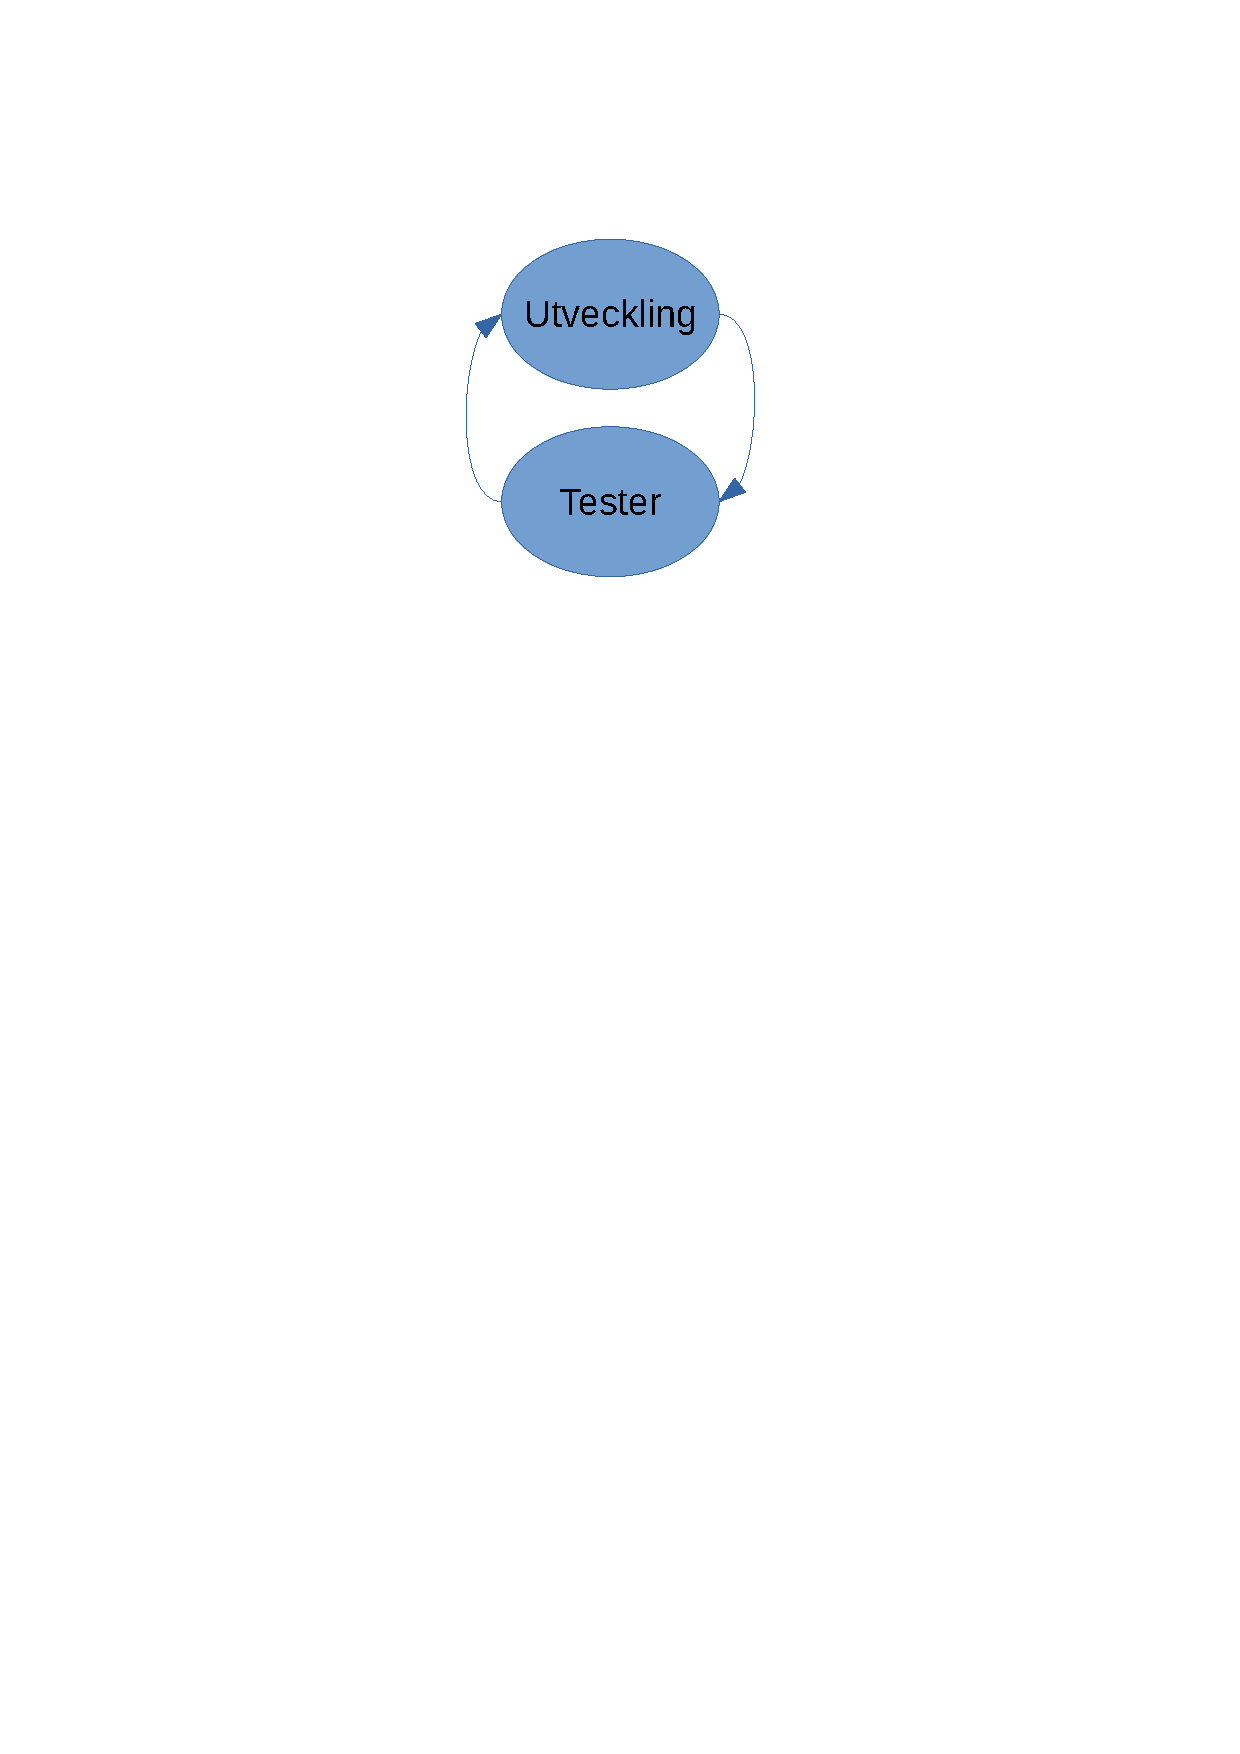
\includegraphics[trim={0 19cm 1cm 3cm}, clip, scale=0.5]{figurer/arbetsrutin.pdf}
  \caption{Vår arbetsrutin. Utvecklarna får direkt återkoppling från testresultaten och kan lösa buggar tidigt i utvecklingsfasen.}
\end{figure}

\end{document}

